\documentclass[oneside,14pt]{extarticle}
\usepackage[utf8]{inputenc}
\usepackage[english,ukrainian]{babel}
\usepackage{amssymb,amsfonts,amsmath,amsthm,mathtext,textcomp}

\usepackage[includehead, headsep=0pt, footskip=0pt, top=2cm, bottom=2cm, left=2cm, right=1cm]{geometry}
\usepackage{indentfirst}
\usepackage[onehalfspacing]{setspace}
\usepackage[headings]{fancyhdr}
\usepackage{etoolbox}
\usepackage{flafter}
\usepackage{listings}
\usepackage{graphicx}
\usepackage{float}
\usepackage[labelsep=period]{caption}

\usepackage{array}
\fancyhf{}
\renewcommand{\headrulewidth}{0pt}
\pagestyle{fancy}
\fancyfoot[R]{\thepage}
\lstset{breaklines=true,}
\graphicspath{ {./pictures} }

\lstset{
	language=c,
	tabsize=4,
	keepspaces,
	showstringspaces=false,
}
\graphicspath{ {./pictures} }
\setlength{\parindent}{4em}

\newcommand\subject{Моделювання та аналіз програмного забезпечення}
\newcommand\lecturer{доцент кафедри ПЗ \\ Сердюк П.В.}
\newcommand\teacher{викладач кафедри ПЗ \\ Микуляк А.В.}
\newcommand\mygroup{ПЗ-22}
\newcommand\lab{1}
\newcommand\theme{Налаштування Git}
\newcommand\purpose{Навчитися налаштовувати та використовувати Git}

\begin{document}
\begin{normalsize}
	\begin{titlepage}
		\thispagestyle{empty}
		\begin{center}
			\textbf{МІНІСТЕРСТВО ОСВІТИ І НАУКИ УКРАЇНИ\\
				НАЦІОНАЛЬНИЙ УНІВЕРСИТЕТ "ЛЬВІВСЬКА ПОЛІТЕХНІКА"}
		\end{center}
		\begin{flushright}
			\textbf{ІКНІ}\\
			Кафедра \textbf{ПЗ}
		\end{flushright}
		\vspace{70pt}
		\begin{center}
			\textbf{ЗВІТ}\\
			\vspace{10pt}
			до лабораторної роботи № \lab\\
			\textbf{на тему}: “\textit{\theme}”\\
			\textbf{з дисципліни}: “\subject”
		\end{center}
		\vspace{50pt}
		\begin{flushright}
			
			\textbf{Лектор}:\\
			\lecturer\\
			\vspace{10pt}
			\textbf{Виконав}:\\
			
			студент групи \mygroup\\
			Коваленко Д.М.\\
			\vspace{10pt}
			\textbf{Прийняв}:\\
			
			\teacher\\
			
			\vspace{28pt}
			«\rule{1cm}{0.15mm}» \rule{1.5cm}{0.15mm} 2023 р.\\
			$\sum$ = \rule{1cm}{0.15mm}……………\\
			
		\end{flushright}
		\vspace{\fill}
		\begin{center}
			\textbf{Львів — 2023}
		\end{center}
	\end{titlepage}
		
	\begin{description}
		\item[Тема.] \theme.
		\item[Мета.] \purpose.
	\end{description}

	\section*{Завдання}
	\begin{enumerate}
		\item Переглянути відео
		
		\item Створити аккаунт створювати на GitLab (тільки GitLab - не GitHub, і не жоден
		інший).
		
		\item Створити репозиторій назвати MAPZ (тільки така назва).
		
		\item Створити папку для лабораторних на компютері. Запустити там git clone для
		репозиторію
		git clone [url репозиторію]
		
		\item Створити структура папок локально на компютері- верхня MAPZ, всередині
		Lab1, Lab2 ,.....
		
		\item Надати доступ до вашого репозиторію pavlo\_serdyuk, з правами доступу до
		коду (низькі права не дозволяють переглядати код).
		
		\item Додати посилання на ваш репозиторійу spreadsheet файл, доступ до кого має
		забезпечити староста групи.
		
		\item Проробити усі дії на сайті https://learngitbranching.js.org/ до 5 рівня (Advanced
		не потрібно) і повторити їх у себе локально на комп’ютері.
		
		\item Усі дії робити у папці Lab1. Для комітів використовувати текстові файли, щоб
		зробити новий коміт, достатньо змінити лінійку тексту всередині файлу.
		
		\item Для кожного завдання використовуйте новий текстовий файл.
		
		\item Звіти повинні містити скріншоти з усіма виконаними операціями (як завдань на
		сайті, так і локального виконання). Додатково до цього можна використати лог,
		що відобразить історію, або будь-яку візуальну надбудову Git - GitKraken,
		SourceTree, TortoiseGit.
		
		\item Звіти завантажити на ВНС
	\end{enumerate}

	\section*{Хід виконання}
		\begin{figure}[H]
			\centering
			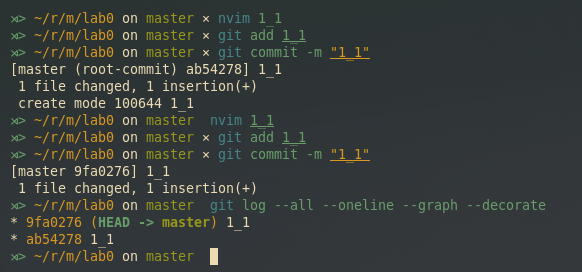
\includegraphics[scale=0.6]{1_1}
			\caption{Виконання завдання 1.1}
		\end{figure}
		\begin{figure}[H]
			\centering
			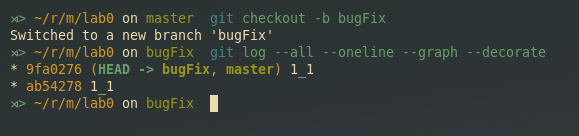
\includegraphics[scale=0.6]{1_2}
			\caption{Виконання завдання 1.2}
		\end{figure}
				\begin{figure}[H]
			\centering
			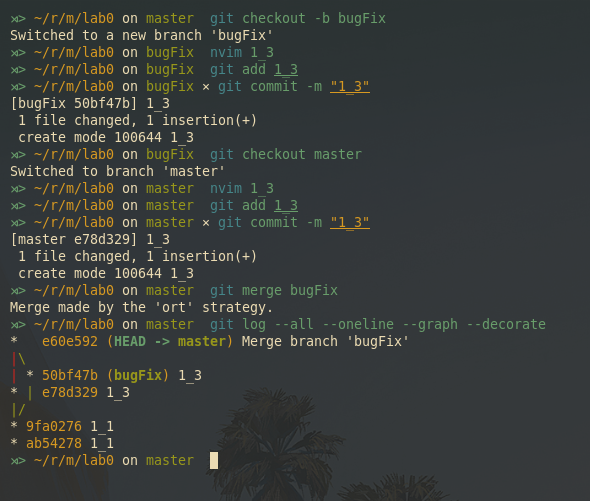
\includegraphics[scale=0.6]{1_3}
			\caption{Виконання завдання 1.3}
		\end{figure}
				\begin{figure}[H]
			\centering
			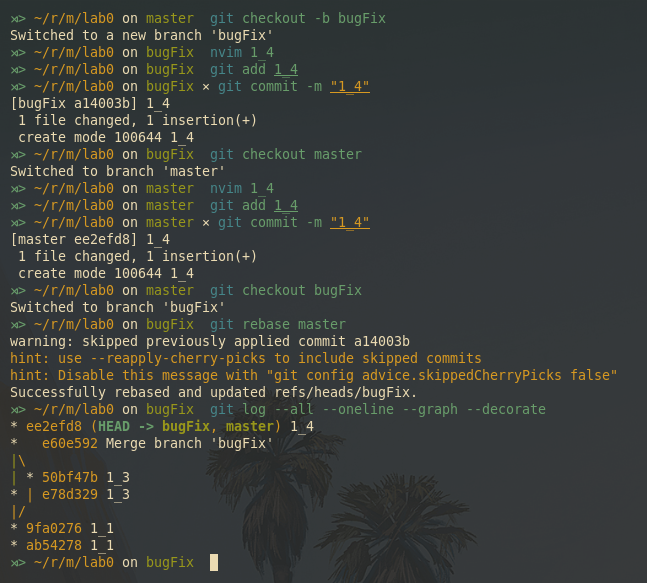
\includegraphics[scale=0.6]{1_4}
			\caption{Виконання завдання 1.4}
		\end{figure}
				\begin{figure}[H]
			\centering
			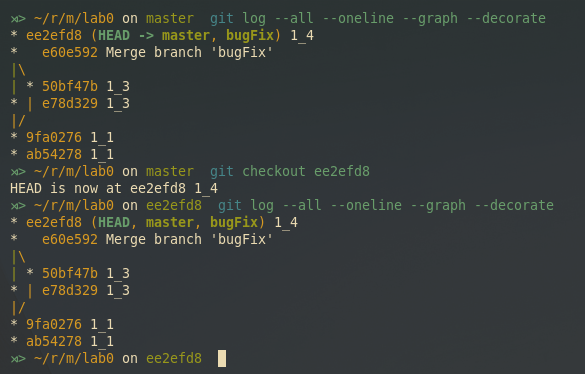
\includegraphics[scale=0.6]{2_1}
			\caption{Виконання завдання 2.1}
		\end{figure}
				\begin{figure}[H]
			\centering
			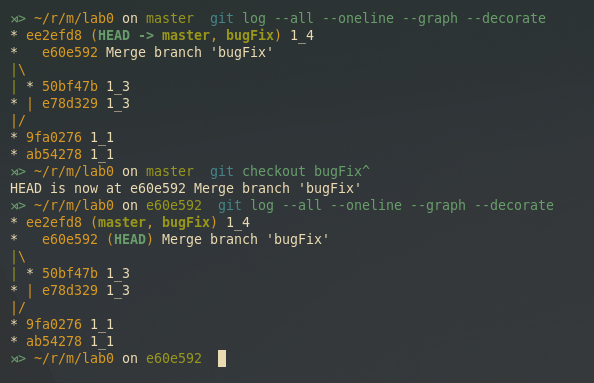
\includegraphics[scale=0.6]{2_2}
			\caption{Виконання завдання 2.2}
		\end{figure}
				\begin{figure}[H]
			\centering
			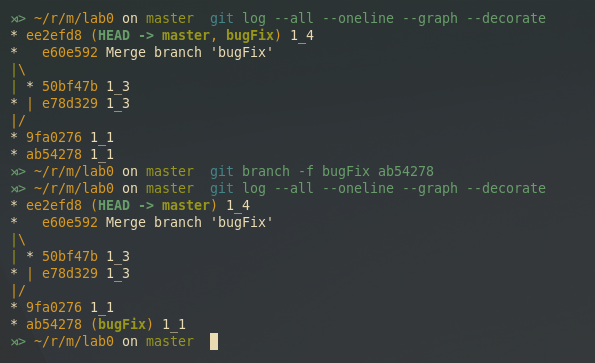
\includegraphics[scale=0.6]{2_3}
			\caption{Виконання завдання 2.3}
		\end{figure}
				\begin{figure}[H]
			\centering
			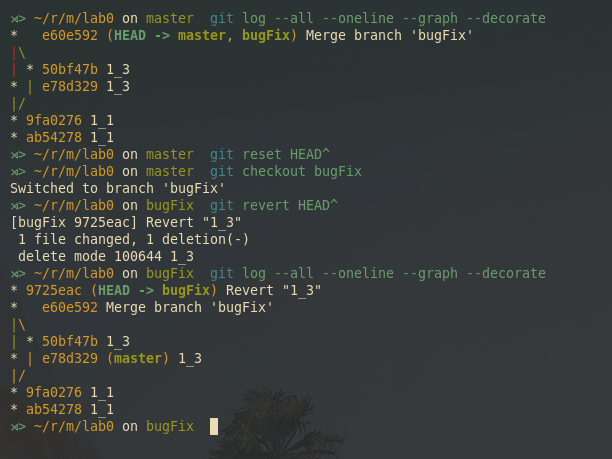
\includegraphics[scale=0.6]{2_4}
			\caption{Виконання завдання 2.4}
		\end{figure}
				\begin{figure}[H]
			\centering
			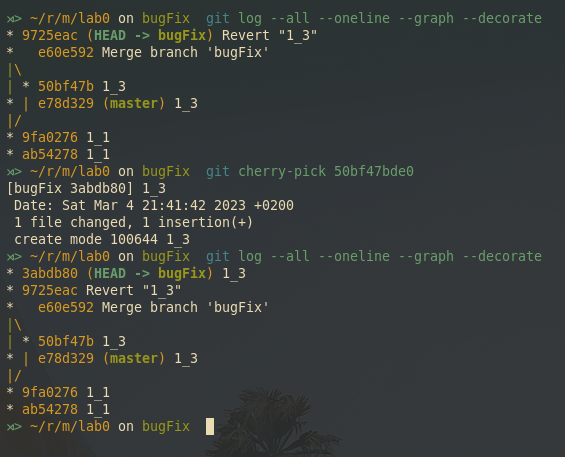
\includegraphics[scale=0.6]{3_1}
			\caption{Виконання завдання 3.1}
		\end{figure}
				\begin{figure}[H]
			\centering
			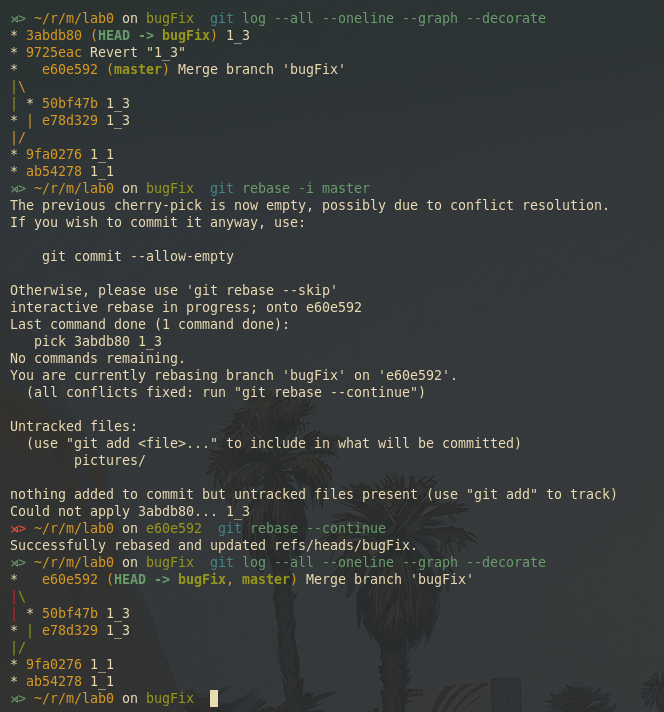
\includegraphics[scale=0.6]{3_2}
			\caption{Виконання завдання 3.2}
		\end{figure}
		\begin{figure}[H]
			\centering
			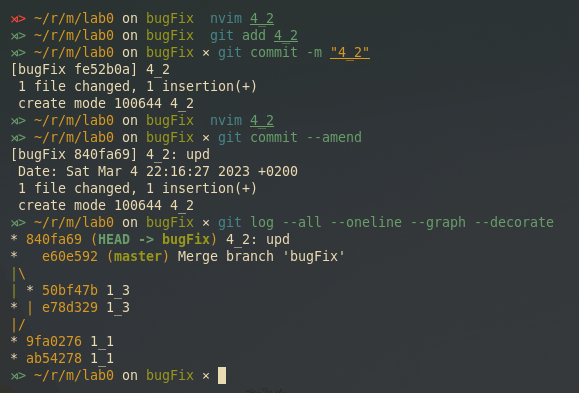
\includegraphics[scale=0.6]{4_2}
			\caption{Виконання завдання 4.2}
		\end{figure}
		\begin{figure}[H]
			\centering
			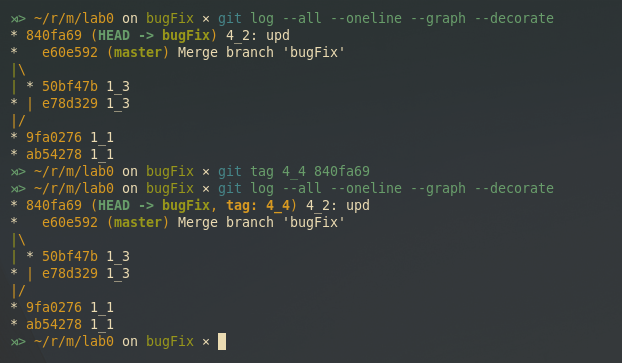
\includegraphics[scale=0.6]{4_3}
			\caption{Виконання завдання 4.3}
		\end{figure}
		\begin{figure}[H]
			\centering
			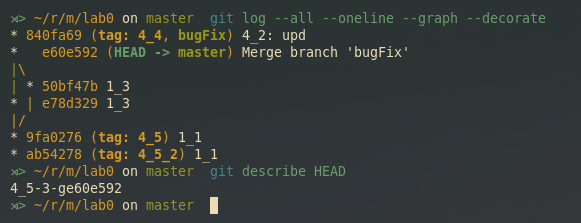
\includegraphics[scale=0.6]{4_5}
			\caption{Виконання завдання 4.5}
		\end{figure}
		
	\section*{Результати}
		\begin{figure}[H]
			\centering
			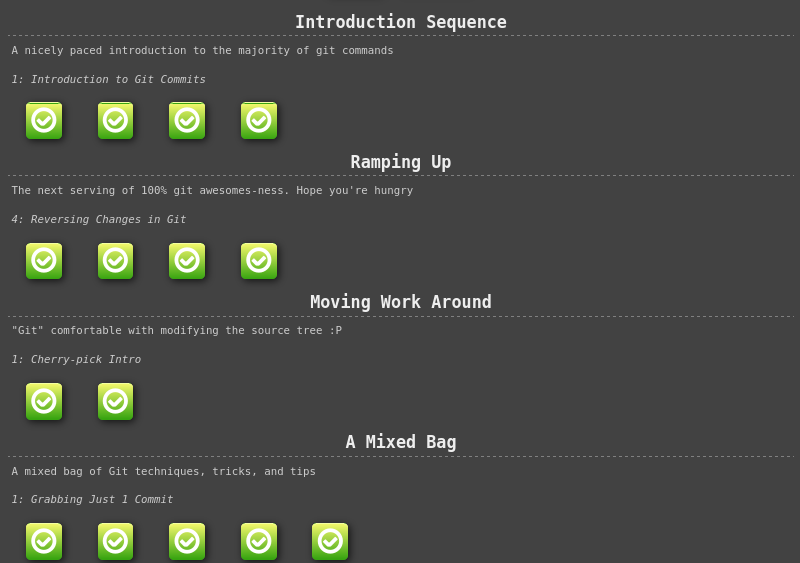
\includegraphics[scale=0.6]{1}
			\caption{Виконання усіх завдання}
		\end{figure}
	\section*{Висновки}
	Під час виконання лабораторної роботи я навчився створювати акаунт та репозиторій на GitLab, навчився використовувати Git з командами commit, push, checkout, branch, tag, rebase, merge, describe, тощо. Я проробив усі дії на сайті https://learngitbranching.js.org/ до 5 рівня.
	    
\end{normalsize}
\end{document}
